% Options for packages loaded elsewhere
\PassOptionsToPackage{unicode}{hyperref}
\PassOptionsToPackage{hyphens}{url}
%
\documentclass[
]{article}
\usepackage{amsmath,amssymb}
\usepackage{lmodern}
\usepackage{iftex}
\ifPDFTeX
  \usepackage[T1]{fontenc}
  \usepackage[utf8]{inputenc}
  \usepackage{textcomp} % provide euro and other symbols
\else % if luatex or xetex
  \usepackage{unicode-math}
  \defaultfontfeatures{Scale=MatchLowercase}
  \defaultfontfeatures[\rmfamily]{Ligatures=TeX,Scale=1}
\fi
% Use upquote if available, for straight quotes in verbatim environments
\IfFileExists{upquote.sty}{\usepackage{upquote}}{}
\IfFileExists{microtype.sty}{% use microtype if available
  \usepackage[]{microtype}
  \UseMicrotypeSet[protrusion]{basicmath} % disable protrusion for tt fonts
}{}
\makeatletter
\@ifundefined{KOMAClassName}{% if non-KOMA class
  \IfFileExists{parskip.sty}{%
    \usepackage{parskip}
  }{% else
    \setlength{\parindent}{0pt}
    \setlength{\parskip}{6pt plus 2pt minus 1pt}}
}{% if KOMA class
  \KOMAoptions{parskip=half}}
\makeatother
\usepackage{xcolor}
\usepackage[margin=1in]{geometry}
\usepackage{graphicx}
\makeatletter
\def\maxwidth{\ifdim\Gin@nat@width>\linewidth\linewidth\else\Gin@nat@width\fi}
\def\maxheight{\ifdim\Gin@nat@height>\textheight\textheight\else\Gin@nat@height\fi}
\makeatother
% Scale images if necessary, so that they will not overflow the page
% margins by default, and it is still possible to overwrite the defaults
% using explicit options in \includegraphics[width, height, ...]{}
\setkeys{Gin}{width=\maxwidth,height=\maxheight,keepaspectratio}
% Set default figure placement to htbp
\makeatletter
\def\fps@figure{htbp}
\makeatother
\setlength{\emergencystretch}{3em} % prevent overfull lines
\providecommand{\tightlist}{%
  \setlength{\itemsep}{0pt}\setlength{\parskip}{0pt}}
\setcounter{secnumdepth}{-\maxdimen} % remove section numbering
\ifLuaTeX
  \usepackage{selnolig}  % disable illegal ligatures
\fi
\IfFileExists{bookmark.sty}{\usepackage{bookmark}}{\usepackage{hyperref}}
\IfFileExists{xurl.sty}{\usepackage{xurl}}{} % add URL line breaks if available
\urlstyle{same} % disable monospaced font for URLs
\hypersetup{
  pdftitle={About},
  pdfauthor={Yoon Lee},
  hidelinks,
  pdfcreator={LaTeX via pandoc}}

\title{About}
\author{Yoon Lee}
\date{2023-02-04}

\begin{document}
\maketitle

\hypertarget{question}{%
\subsection{Question}\label{question}}

How would the visualization of different skills required for data
scientist roles in companies performing at different Sectors and states
look like? In addition to that, what are the average salaries for
different roles?

\hypertarget{insights}{%
\subsection{Insights}\label{insights}}

Information Technology Sector has the most data science roles of
\textbf{108}. Following up on that, Biotech \& Pharmaceuticals sector
has a role of \textbf{89}, and Business Service has a role of
\textbf{70}.

Within IT sector, \textbf{California} is the most operated state among
companies in IT sector with \textbf{41} jobs available. Surprisingly,
\textbf{New York} only hosts \textbf{7} jobs for IT companies.

These IT companies \textbf{want Python the most} from their employees.
\textbf{SQL and excel} are the \textbf{top 2 \& 3} most wanted skills
from data scientists. 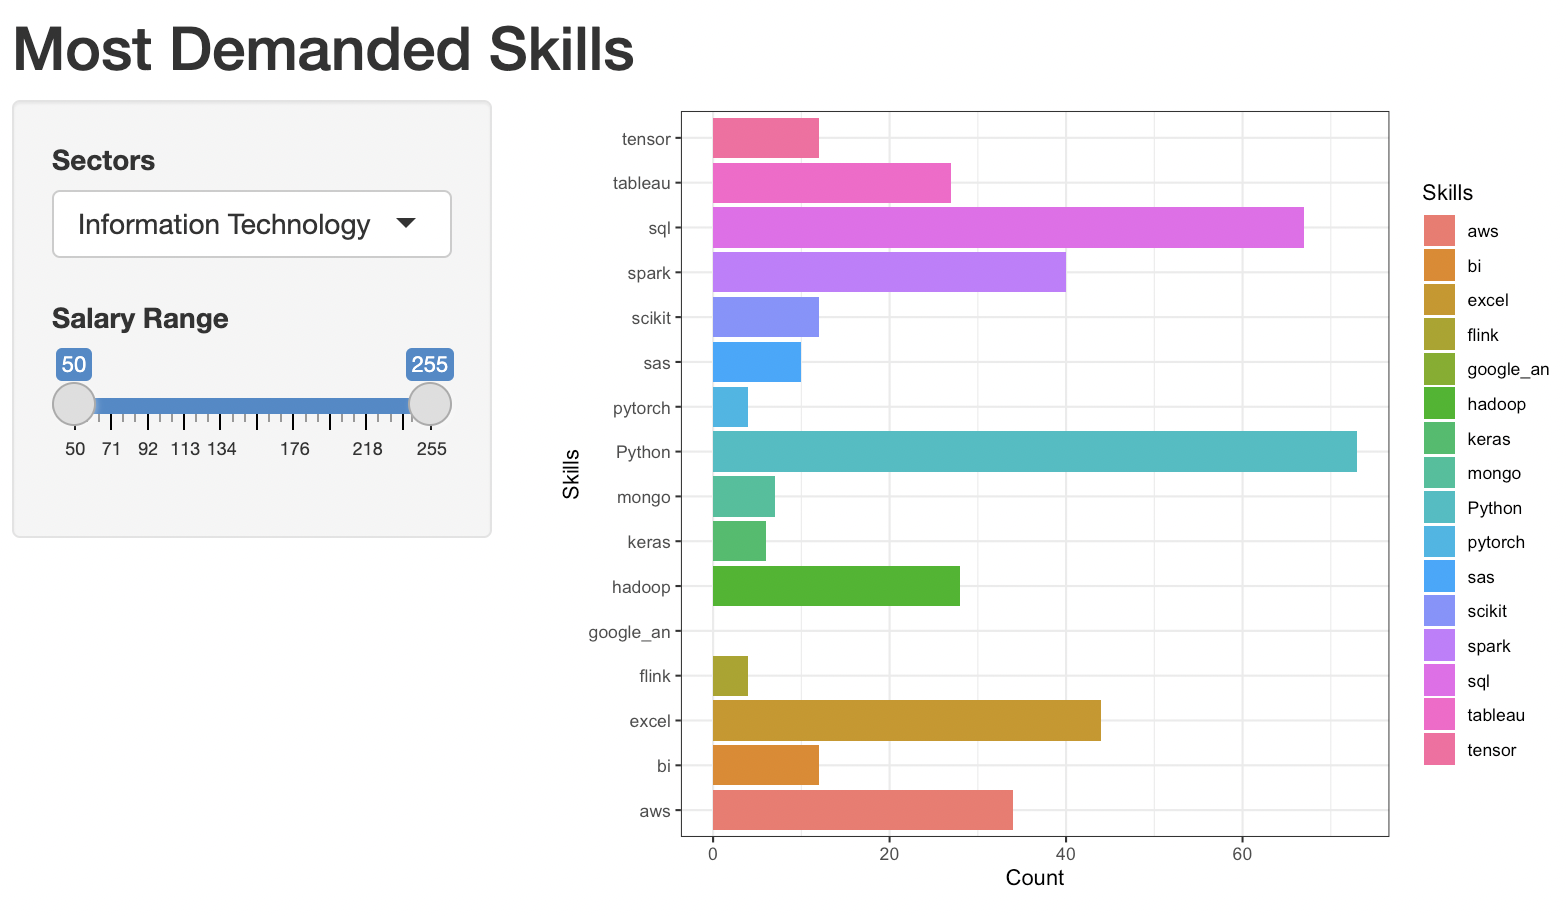
\includegraphics{data/IT-skills.png}

In Biotech \& Pharma, \textbf{43 roles are in Massachusetts}, and
following MA, \textbf{California has 15 roles} available for data
scientists.

Here, companies \textbf{want excel the most} with \textbf{python and AWS
as 2nd and 3rd} most sought-after skills.

\includegraphics{data/Bio\&Pharm-skills.png}

For business service, jobs are more evenly distributed than other two
states: \textbf{9 in CA, 8 in PA, 7 in NY \& TX}.

The most wanted skills are as follows: SQL, Python, Excel.

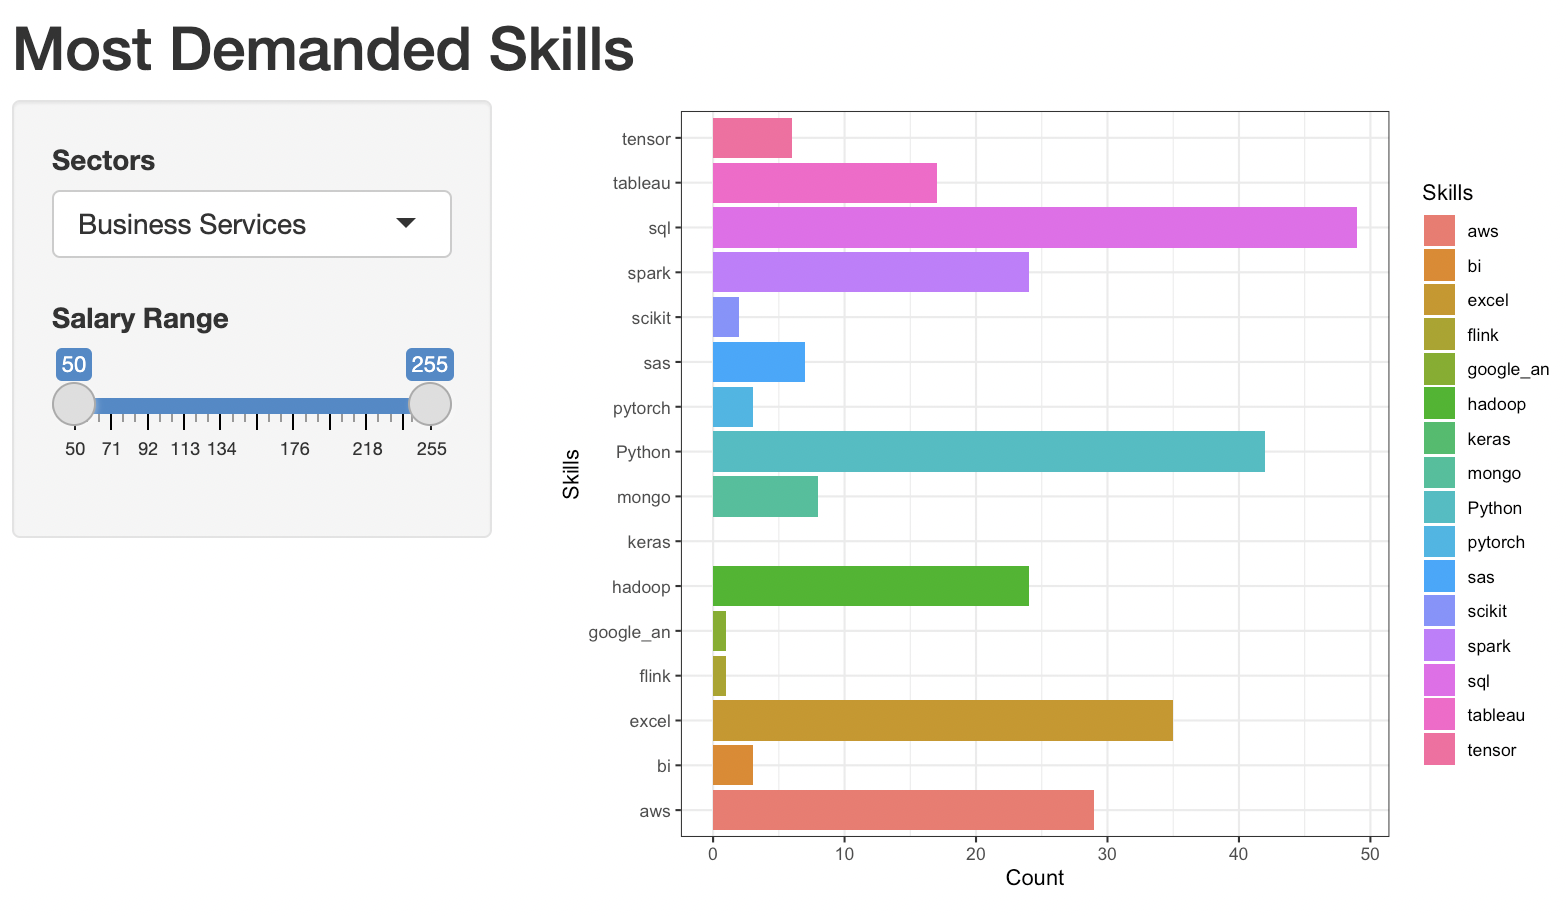
\includegraphics{data/Business_Service-skills.png}

\end{document}
